\documentclass[1p]{elsarticle_modified}
%\bibliographystyle{elsarticle-num}

%\usepackage[colorlinks]{hyperref}
%\usepackage{abbrmath_seonhwa} %\Abb, \Ascr, \Acal ,\Abf, \Afrak
\usepackage{amsfonts}
\usepackage{amssymb}
\usepackage{amsmath}
\usepackage{amsthm}
\usepackage{scalefnt}
\usepackage{amsbsy}
\usepackage{kotex}
\usepackage{caption}
\usepackage{subfig}
\usepackage{color}
\usepackage{graphicx}
\usepackage{xcolor} %% white, black, red, green, blue, cyan, magenta, yellow
\usepackage{float}
\usepackage{setspace}
\usepackage{hyperref}

\usepackage{tikz}
\usetikzlibrary{arrows}

\usepackage{multirow}
\usepackage{array} % fixed length table
\usepackage{hhline}

%%%%%%%%%%%%%%%%%%%%%
\makeatletter
\renewcommand*\env@matrix[1][\arraystretch]{%
	\edef\arraystretch{#1}%
	\hskip -\arraycolsep
	\let\@ifnextchar\new@ifnextchar
	\array{*\c@MaxMatrixCols c}}
\makeatother %https://tex.stackexchange.com/questions/14071/how-can-i-increase-the-line-spacing-in-a-matrix
%%%%%%%%%%%%%%%

\usepackage[normalem]{ulem}

\newcommand{\msout}[1]{\ifmmode\text{\sout{\ensuremath{#1}}}\else\sout{#1}\fi}
%SOURCE: \msout is \stkout macro in https://tex.stackexchange.com/questions/20609/strikeout-in-math-mode

\newcommand{\cancel}[1]{
	\ifmmode
	{\color{red}\msout{#1}}
	\else
	{\color{red}\sout{#1}}
	\fi
}

\newcommand{\add}[1]{
	{\color{blue}\uwave{#1}}
}

\newcommand{\replace}[2]{
	\ifmmode
	{\color{red}\msout{#1}}{\color{blue}\uwave{#2}}
	\else
	{\color{red}\sout{#1}}{\color{blue}\uwave{#2}}
	\fi
}

\newcommand{\Sol}{\mathcal{S}} %segment
\newcommand{\D}{D} %diagram
\newcommand{\A}{\mathcal{A}} %arc


%%%%%%%%%%%%%%%%%%%%%%%%%%%%%5 test

\def\sl{\operatorname{\textup{SL}}(2,\Cbb)}
\def\psl{\operatorname{\textup{PSL}}(2,\Cbb)}
\def\quan{\mkern 1mu \triangleright \mkern 1mu}

\theoremstyle{definition}
\newtheorem{thm}{Theorem}[section]
\newtheorem{prop}[thm]{Proposition}
\newtheorem{lem}[thm]{Lemma}
\newtheorem{ques}[thm]{Question}
\newtheorem{cor}[thm]{Corollary}
\newtheorem{defn}[thm]{Definition}
\newtheorem{exam}[thm]{Example}
\newtheorem{rmk}[thm]{Remark}
\newtheorem{alg}[thm]{Algorithm}

\newcommand{\I}{\sqrt{-1}}
\begin{document}

%\begin{frontmatter}
%
%\title{Boundary parabolic representations of knots up to 8 crossings}
%
%%% Group authors per affiliation:
%\author{Yunhi Cho} 
%\address{Department of Mathematics, University of Seoul, Seoul, Korea}
%\ead{yhcho@uos.ac.kr}
%
%
%\author{Seonhwa Kim} %\fnref{s_kim}}
%\address{Center for Geometry and Physics, Institute for Basic Science, Pohang, 37673, Korea}
%\ead{ryeona17@ibs.re.kr}
%
%\author{Hyuk Kim}
%\address{Department of Mathematical Sciences, Seoul National University, Seoul 08826, Korea}
%\ead{hyukkim@snu.ac.kr}
%
%\author{Seokbeom Yoon}
%\address{Department of Mathematical Sciences, Seoul National University, Seoul, 08826,  Korea}
%\ead{sbyoon15@snu.ac.kr}
%
%\begin{abstract}
%We find all boundary parabolic representation of knots up to 8 crossings.
%
%\end{abstract}
%\begin{keyword}
%    \MSC[2010] 57M25 
%\end{keyword}
%
%\end{frontmatter}

%\linenumbers
%\tableofcontents
%
\newcommand\colored[1]{\textcolor{white}{\rule[-0.35ex]{0.8em}{1.4ex}}\kern-0.8em\color{red} #1}%
%\newcommand\colored[1]{\textcolor{white}{ #1}\kern-2.17ex	\textcolor{white}{ #1}\kern-1.81ex	\textcolor{white}{ #1}\kern-2.15ex\color{red}#1	}

{\Large $\underline{12a_{0808}~(K12a_{0808})}$}

\setlength{\tabcolsep}{10pt}
\renewcommand{\arraystretch}{1.6}
\vspace{1cm}\begin{tabular}{m{100pt}>{\centering\arraybackslash}m{274pt}}
\multirow{5}{120pt}{
	\centering
	\includegraphics[width=112pt]{../../../GIT/diagram.site/Diagrams/png/1609_12a_0808.png}\\
\ \ \ A knot diagram\footnotemark}&
\allowdisplaybreaks
\textbf{Linearized knot diagam} \\
\cline{2-2}
 &
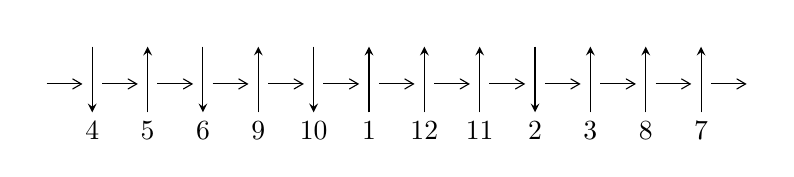
\begin{tikzpicture}[x=20pt, y=17pt]
	% nodes
	\node (C0) at (0, 0) {};
	\node (C1) at (1, 0) {};
	\node (C1U) at (1, +1) {};
	\node (C1D) at (1, -1) {4};

	\node (C2) at (2, 0) {};
	\node (C2U) at (2, +1) {};
	\node (C2D) at (2, -1) {5};

	\node (C3) at (3, 0) {};
	\node (C3U) at (3, +1) {};
	\node (C3D) at (3, -1) {6};

	\node (C4) at (4, 0) {};
	\node (C4U) at (4, +1) {};
	\node (C4D) at (4, -1) {9};

	\node (C5) at (5, 0) {};
	\node (C5U) at (5, +1) {};
	\node (C5D) at (5, -1) {10};

	\node (C6) at (6, 0) {};
	\node (C6U) at (6, +1) {};
	\node (C6D) at (6, -1) {1};

	\node (C7) at (7, 0) {};
	\node (C7U) at (7, +1) {};
	\node (C7D) at (7, -1) {12};

	\node (C8) at (8, 0) {};
	\node (C8U) at (8, +1) {};
	\node (C8D) at (8, -1) {11};

	\node (C9) at (9, 0) {};
	\node (C9U) at (9, +1) {};
	\node (C9D) at (9, -1) {2};

	\node (C10) at (10, 0) {};
	\node (C10U) at (10, +1) {};
	\node (C10D) at (10, -1) {3};

	\node (C11) at (11, 0) {};
	\node (C11U) at (11, +1) {};
	\node (C11D) at (11, -1) {8};

	\node (C12) at (12, 0) {};
	\node (C12U) at (12, +1) {};
	\node (C12D) at (12, -1) {7};
	\node (C13) at (13, 0) {};

	% arrows
	\draw[->,>={angle 60}]
	(C0) edge (C1) (C1) edge (C2) (C2) edge (C3) (C3) edge (C4) (C4) edge (C5) (C5) edge (C6) (C6) edge (C7) (C7) edge (C8) (C8) edge (C9) (C9) edge (C10) (C10) edge (C11) (C11) edge (C12) (C12) edge (C13) ;	\draw[->,>=stealth]
	(C1U) edge (C1D) (C2D) edge (C2U) (C3U) edge (C3D) (C4D) edge (C4U) (C5U) edge (C5D) (C6D) edge (C6U) (C7D) edge (C7U) (C8D) edge (C8U) (C9U) edge (C9D) (C10D) edge (C10U) (C11D) edge (C11U) (C12D) edge (C12U) ;
	\end{tikzpicture} \\
\hhline{~~} \\& 
\textbf{Solving Sequence} \\ \cline{2-2} 
 &
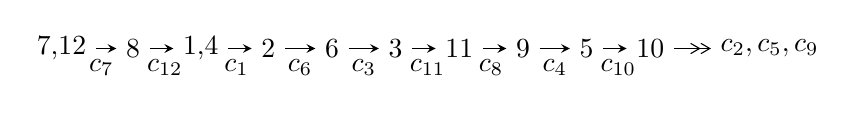
\begin{tikzpicture}[x=23pt, y=7pt]
	% node
	\node (A0) at (-1/8, 0) {7,12};
	\node (A1) at (1, 0) {8};
	\node (A2) at (33/16, 0) {1,4};
	\node (A3) at (25/8, 0) {2};
	\node (A4) at (33/8, 0) {6};
	\node (A5) at (41/8, 0) {3};
	\node (A6) at (49/8, 0) {11};
	\node (A7) at (57/8, 0) {9};
	\node (A8) at (65/8, 0) {5};
	\node (A9) at (73/8, 0) {10};
	\node (C1) at (1/2, -1) {$c_{7}$};
	\node (C2) at (3/2, -1) {$c_{12}$};
	\node (C3) at (21/8, -1) {$c_{1}$};
	\node (C4) at (29/8, -1) {$c_{6}$};
	\node (C5) at (37/8, -1) {$c_{3}$};
	\node (C6) at (45/8, -1) {$c_{11}$};
	\node (C7) at (53/8, -1) {$c_{8}$};
	\node (C8) at (61/8, -1) {$c_{4}$};
	\node (C9) at (69/8, -1) {$c_{10}$};
	\node (A10) at (11, 0) {$c_{2},c_{5},c_{9}$};

	% edge
	\draw[->,>=stealth]	
	(A0) edge (A1) (A1) edge (A2) (A2) edge (A3) (A3) edge (A4) (A4) edge (A5) (A5) edge (A6) (A6) edge (A7) (A7) edge (A8) (A8) edge (A9) ;
	\draw[->>,>={angle 60}]	
	(A9) edge (A10);
\end{tikzpicture} \\ 

\end{tabular} \\

\footnotetext{
The image of knot diagram is generated by the software ``\textbf{Draw programme}" developed by Andrew Bartholomew(\url{http://www.layer8.co.uk/maths/draw/index.htm\#Running-draw}), where we modified some parts for our purpose(\url{https://github.com/CATsTAILs/LinksPainter}).
}\phantom \\ \newline 
\centering \textbf{Ideals for irreducible components\footnotemark of $X_{\text{par}}$} 
 
\begin{align*}
I^u_{1}&=\langle 
-4708 u^{36}+22559 u^{35}+\cdots+12181 b+159188,\\
\phantom{I^u_{1}}&\phantom{= \langle  }184180 u^{36}-854911 u^{35}+\cdots+133991 a-2353969,\;u^{37}-5 u^{36}+\cdots-93 u+11\rangle \\
I^u_{2}&=\langle 
11 u^{22} a+26 u^{22}+\cdots+4 a+1,\;u^{22}+4 u^{21}+\cdots+a-4,\;u^{23}+3 u^{22}+\cdots-6 u^2+1\rangle \\
I^u_{3}&=\langle 
u^{10}+3 u^9+10 u^8+20 u^7+33 u^6+43 u^5+42 u^4+32 u^3+17 u^2+b+6 u+1,\\
\phantom{I^u_{3}}&\phantom{= \langle  }- u^{13}-2 u^{12}-12 u^{11}-19 u^{10}-53 u^9-65 u^8-106 u^7-95 u^6-93 u^5-52 u^4-27 u^3-3 u^2+a+3,\\
\phantom{I^u_{3}}&\phantom{= \langle  }u^{14}+2 u^{13}+\cdots+3 u+1\rangle \\
\\
I^v_{1}&=\langle 
a,\;b-1,\;v-1\rangle \\
\end{align*}
\raggedright * 4 irreducible components of $\dim_{\mathbb{C}}=0$, with total 98 representations.\\
\footnotetext{All coefficients of polynomials are rational numbers. But the coefficients are sometimes approximated in decimal forms when there is not enough margin.}
\newpage
\renewcommand{\arraystretch}{1}
\centering \section*{I. $I^u_{1}= \langle -4708 u^{36}+22559 u^{35}+\cdots+12181 b+159188,\;1.84\times10^{5} u^{36}-8.55\times10^{5} u^{35}+\cdots+1.34\times10^{5} a-2.35\times10^{6},\;u^{37}-5 u^{36}+\cdots-93 u+11 \rangle$}
\flushleft \textbf{(i) Arc colorings}\\
\begin{tabular}{m{7pt} m{180pt} m{7pt} m{180pt} }
\flushright $a_{7}=$&$\begin{pmatrix}1\\0\end{pmatrix}$ \\
\flushright $a_{12}=$&$\begin{pmatrix}0\\u\end{pmatrix}$ \\
\flushright $a_{8}=$&$\begin{pmatrix}1\\- u^2\end{pmatrix}$ \\
\flushright $a_{1}=$&$\begin{pmatrix}u\\u\end{pmatrix}$ \\
\flushright $a_{4}=$&$\begin{pmatrix}-1.37457 u^{36}+6.38036 u^{35}+\cdots-159.292 u+17.5681\\0.386504 u^{36}-1.85198 u^{35}+\cdots+99.2238 u-13.0685\end{pmatrix}$ \\
\flushright $a_{2}=$&$\begin{pmatrix}-3.17294 u^{36}+14.8917 u^{35}+\cdots-300.428 u+33.3318\\0.892455 u^{36}-4.15631 u^{35}+\cdots+240.876 u-30.6508\end{pmatrix}$ \\
\flushright $a_{6}=$&$\begin{pmatrix}u^2+1\\u^2\end{pmatrix}$ \\
\flushright $a_{3}=$&$\begin{pmatrix}-0.695562 u^{36}+3.44817 u^{35}+\cdots-15.1053 u-3.85542\\0.492488 u^{36}-2.10557 u^{35}+\cdots+110.267 u-15.1203\end{pmatrix}$ \\
\flushright $a_{11}=$&$\begin{pmatrix}- u\\u^3+u\end{pmatrix}$ \\
\flushright $a_{9}=$&$\begin{pmatrix}u^2+1\\- u^4-2 u^2\end{pmatrix}$ \\
\flushright $a_{5}=$&$\begin{pmatrix}-0.800315 u^{36}+3.60432 u^{35}+\cdots-74.9791 u+8.59307\\0.134143 u^{36}-0.748543 u^{35}+\cdots+43.9825 u-4.57902\end{pmatrix}$ \\
\flushright $a_{10}=$&$\begin{pmatrix}1.44794 u^{36}-6.84097 u^{35}+\cdots+204.364 u-29.2190\\0.0802890 u^{36}-0.953534 u^{35}+\cdots+17.4424 u+1.26911\end{pmatrix}$\\&\end{tabular}
\flushleft \textbf{(ii) Obstruction class $= -1$}\\~\\
\flushleft \textbf{(iii) Cusp Shapes $= \frac{56806}{12181} u^{36}-\frac{266817}{12181} u^{35}+\cdots+\frac{12593355}{12181} u-\frac{1834736}{12181}$}\\~\\
\newpage\renewcommand{\arraystretch}{1}
\flushleft \textbf{(iv) u-Polynomials at the component}\newline \\
\begin{tabular}{m{50pt}|m{274pt}}
Crossings & \hspace{64pt}u-Polynomials at each crossing \\
\hline $$\begin{aligned}c_{1},c_{3}\end{aligned}$$&$\begin{aligned}
&u^{37}+4 u^{36}+\cdots+24 u-1
\end{aligned}$\\
\hline $$\begin{aligned}c_{2}\end{aligned}$$&$\begin{aligned}
&u^{37}+22 u^{36}+\cdots-87 u-11
\end{aligned}$\\
\hline $$\begin{aligned}c_{4},c_{10}\end{aligned}$$&$\begin{aligned}
&u^{37}+2 u^{35}+\cdots-31 u^2-3
\end{aligned}$\\
\hline $$\begin{aligned}c_{5},c_{9}\end{aligned}$$&$\begin{aligned}
&u^{37}- u^{36}+\cdots+3 u-1
\end{aligned}$\\
\hline $$\begin{aligned}c_{6},c_{7},c_{8}\\c_{11},c_{12}\end{aligned}$$&$\begin{aligned}
&u^{37}+5 u^{36}+\cdots-93 u-11
\end{aligned}$\\
\hline
\end{tabular}\\~\\
\newpage\renewcommand{\arraystretch}{1}
\flushleft \textbf{(v) Riley Polynomials at the component}\newline \\
\begin{tabular}{m{50pt}|m{274pt}}
Crossings & \hspace{64pt}Riley Polynomials at each crossing \\
\hline $$\begin{aligned}c_{1},c_{3}\end{aligned}$$&$\begin{aligned}
&y^{37}-32 y^{36}+\cdots+114 y-1
\end{aligned}$\\
\hline $$\begin{aligned}c_{2}\end{aligned}$$&$\begin{aligned}
&y^{37}+46 y^{35}+\cdots+419 y-121
\end{aligned}$\\
\hline $$\begin{aligned}c_{4},c_{10}\end{aligned}$$&$\begin{aligned}
&y^{37}+4 y^{36}+\cdots-186 y-9
\end{aligned}$\\
\hline $$\begin{aligned}c_{5},c_{9}\end{aligned}$$&$\begin{aligned}
&y^{37}-15 y^{36}+\cdots+39 y-1
\end{aligned}$\\
\hline $$\begin{aligned}c_{6},c_{7},c_{8}\\c_{11},c_{12}\end{aligned}$$&$\begin{aligned}
&y^{37}+51 y^{36}+\cdots+245 y-121
\end{aligned}$\\
\hline
\end{tabular}\\~\\
\newpage\flushleft \textbf{(vi) Complex Volumes and Cusp Shapes}
$$\begin{array}{c|c|c}  
\text{Solutions to }I^u_{1}& \I (\text{vol} + \sqrt{-1}CS) & \text{Cusp shape}\\
 \hline 
\begin{aligned}
u &= -0.024756 + 1.003880 I \\
a &= \phantom{-}1.175790 - 0.520011 I \\
b &= \phantom{-}0.66374 - 1.62745 I\end{aligned}
 & -5.00500 - 0.12327 I & -5.98815 + 0. I\phantom{ +0.000000I} \\ \hline\begin{aligned}
u &= -0.024756 - 1.003880 I \\
a &= \phantom{-}1.175790 + 0.520011 I \\
b &= \phantom{-}0.66374 + 1.62745 I\end{aligned}
 & -5.00500 + 0.12327 I & -5.98815 + 0. I\phantom{ +0.000000I} \\ \hline\begin{aligned}
u &= \phantom{-}0.289437 + 0.983506 I \\
a &= \phantom{-}0.571567 - 0.060773 I \\
b &= \phantom{-}0.93730 - 1.28805 I\end{aligned}
 & -5.74342 + 2.02777 I & -6.65386 - 1.42849 I \\ \hline\begin{aligned}
u &= \phantom{-}0.289437 - 0.983506 I \\
a &= \phantom{-}0.571567 + 0.060773 I \\
b &= \phantom{-}0.93730 + 1.28805 I\end{aligned}
 & -5.74342 - 2.02777 I & -6.65386 + 1.42849 I \\ \hline\begin{aligned}
u &= \phantom{-}0.255241 + 1.040160 I \\
a &= \phantom{-}0.614543 - 0.711849 I \\
b &= \phantom{-}0.02855 - 2.23185 I\end{aligned}
 & -6.18042 + 5.52248 I & -8.08952 - 8.67422 I \\ \hline\begin{aligned}
u &= \phantom{-}0.255241 - 1.040160 I \\
a &= \phantom{-}0.614543 + 0.711849 I \\
b &= \phantom{-}0.02855 + 2.23185 I\end{aligned}
 & -6.18042 - 5.52248 I & -8.08952 + 8.67422 I \\ \hline\begin{aligned}
u &= -0.174584 + 0.835928 I \\
a &= -0.438786 + 0.614183 I \\
b &= \phantom{-}0.159818 + 0.734522 I\end{aligned}
 & -1.41316 - 2.04594 I & \phantom{-}1.13419 + 3.99911 I \\ \hline\begin{aligned}
u &= -0.174584 - 0.835928 I \\
a &= -0.438786 - 0.614183 I \\
b &= \phantom{-}0.159818 - 0.734522 I\end{aligned}
 & -1.41316 + 2.04594 I & \phantom{-}1.13419 - 3.99911 I \\ \hline\begin{aligned}
u &= \phantom{-}0.373017 + 1.086120 I \\
a &= -0.263327 + 0.662536 I \\
b &= \phantom{-}0.03559 + 2.06531 I\end{aligned}
 & -5.4061 + 14.0876 I & \phantom{-0.000000 } 0 \\ \hline\begin{aligned}
u &= \phantom{-}0.373017 - 1.086120 I \\
a &= -0.263327 - 0.662536 I \\
b &= \phantom{-}0.03559 - 2.06531 I\end{aligned}
 & -5.4061 - 14.0876 I & \phantom{-0.000000 } 0\\
 \hline 
 \end{array}$$\newpage$$\begin{array}{c|c|c}  
\text{Solutions to }I^u_{1}& \I (\text{vol} + \sqrt{-1}CS) & \text{Cusp shape}\\
 \hline 
\begin{aligned}
u &= \phantom{-}0.601924 + 0.470380 I \\
a &= \phantom{-}0.819217 - 0.043610 I \\
b &= -0.639760 + 0.296764 I\end{aligned}
 & -1.57344 - 6.55157 I & \phantom{-}0.66439 + 4.08814 I \\ \hline\begin{aligned}
u &= \phantom{-}0.601924 - 0.470380 I \\
a &= \phantom{-}0.819217 + 0.043610 I \\
b &= -0.639760 - 0.296764 I\end{aligned}
 & -1.57344 + 6.55157 I & \phantom{-}0.66439 - 4.08814 I \\ \hline\begin{aligned}
u &= \phantom{-}0.258979 + 1.229600 I \\
a &= -0.583862 + 0.387661 I \\
b &= -0.797830 + 1.118640 I\end{aligned}
 & -7.04198 - 3.53330 I & \phantom{-0.000000 } 0 \\ \hline\begin{aligned}
u &= \phantom{-}0.258979 - 1.229600 I \\
a &= -0.583862 - 0.387661 I \\
b &= -0.797830 - 1.118640 I\end{aligned}
 & -7.04198 + 3.53330 I & \phantom{-0.000000 } 0 \\ \hline\begin{aligned}
u &= \phantom{-}0.644949 + 0.303940 I \\
a &= \phantom{-}0.889386 - 0.999870 I \\
b &= -0.211320 + 0.616406 I\end{aligned}
 & -1.07949 + 10.62970 I & \phantom{-}2.38501 - 8.97197 I \\ \hline\begin{aligned}
u &= \phantom{-}0.644949 - 0.303940 I \\
a &= \phantom{-}0.889386 + 0.999870 I \\
b &= -0.211320 - 0.616406 I\end{aligned}
 & -1.07949 - 10.62970 I & \phantom{-}2.38501 + 8.97197 I \\ \hline\begin{aligned}
u &= -0.494000 + 0.492655 I \\
a &= -0.382762 + 0.046228 I \\
b &= -0.189464 + 0.141918 I\end{aligned}
 & \phantom{-}0.72150 - 1.71038 I & \phantom{-}5.72840 - 0.24301 I \\ \hline\begin{aligned}
u &= -0.494000 - 0.492655 I \\
a &= -0.382762 - 0.046228 I \\
b &= -0.189464 - 0.141918 I\end{aligned}
 & \phantom{-}0.72150 + 1.71038 I & \phantom{-}5.72840 + 0.24301 I \\ \hline\begin{aligned}
u &= \phantom{-}0.450704 + 0.280399 I \\
a &= -0.64300 + 1.61268 I \\
b &= \phantom{-}0.407710 - 0.737598 I\end{aligned}
 & -2.07909 + 3.10269 I & -2.55857 - 8.69904 I \\ \hline\begin{aligned}
u &= \phantom{-}0.450704 - 0.280399 I \\
a &= -0.64300 - 1.61268 I \\
b &= \phantom{-}0.407710 + 0.737598 I\end{aligned}
 & -2.07909 - 3.10269 I & -2.55857 + 8.69904 I\\
 \hline 
 \end{array}$$\newpage$$\begin{array}{c|c|c}  
\text{Solutions to }I^u_{1}& \I (\text{vol} + \sqrt{-1}CS) & \text{Cusp shape}\\
 \hline 
\begin{aligned}
u &= -0.13418 + 1.50316 I \\
a &= -0.336179 + 0.293626 I \\
b &= -0.297595 + 0.492362 I\end{aligned}
 & -5.92171 - 3.96285 I & \phantom{-0.000000 } 0 \\ \hline\begin{aligned}
u &= -0.13418 - 1.50316 I \\
a &= -0.336179 - 0.293626 I \\
b &= -0.297595 - 0.492362 I\end{aligned}
 & -5.92171 + 3.96285 I & \phantom{-0.000000 } 0 \\ \hline\begin{aligned}
u &= \phantom{-}0.397512 + 0.237116 I \\
a &= -1.54677 + 0.52584 I \\
b &= \phantom{-}0.690346 - 0.066411 I\end{aligned}
 & -2.09954 - 0.39329 I & -2.47917 - 0.74863 I \\ \hline\begin{aligned}
u &= \phantom{-}0.397512 - 0.237116 I \\
a &= -1.54677 - 0.52584 I \\
b &= \phantom{-}0.690346 + 0.066411 I\end{aligned}
 & -2.09954 + 0.39329 I & -2.47917 + 0.74863 I \\ \hline\begin{aligned}
u &= -0.409769\phantom{ +0.000000I} \\
a &= -0.906661\phantom{ +0.000000I} \\
b &= -0.331981\phantom{ +0.000000I}\end{aligned}
 & \phantom{-}1.05211\phantom{ +0.000000I} & \phantom{-}10.2210\phantom{ +0.000000I} \\ \hline\begin{aligned}
u &= -0.03012 + 1.68814 I \\
a &= \phantom{-}0.548995 + 1.286040 I \\
b &= \phantom{-}1.05584 + 1.49435 I\end{aligned}
 & -10.41680 - 2.72771 I & \phantom{-0.000000 } 0 \\ \hline\begin{aligned}
u &= -0.03012 - 1.68814 I \\
a &= \phantom{-}0.548995 - 1.286040 I \\
b &= \phantom{-}1.05584 - 1.49435 I\end{aligned}
 & -10.41680 + 2.72771 I & \phantom{-0.000000 } 0 \\ \hline\begin{aligned}
u &= \phantom{-}0.08129 + 1.71808 I \\
a &= \phantom{-}1.09520 - 1.84279 I \\
b &= \phantom{-}1.02527 - 2.70249 I\end{aligned}
 & -15.3380 + 3.5515 I & \phantom{-0.000000 } 0 \\ \hline\begin{aligned}
u &= \phantom{-}0.08129 - 1.71808 I \\
a &= \phantom{-}1.09520 + 1.84279 I \\
b &= \phantom{-}1.02527 + 2.70249 I\end{aligned}
 & -15.3380 - 3.5515 I & \phantom{-0.000000 } 0 \\ \hline\begin{aligned}
u &= -0.00798 + 1.73092 I \\
a &= \phantom{-}0.42758 - 2.20249 I \\
b &= -0.00155 - 2.93076 I\end{aligned}
 & -14.8725 - 0.2681 I & \phantom{-0.000000 } 0\\
 \hline 
 \end{array}$$\newpage$$\begin{array}{c|c|c}  
\text{Solutions to }I^u_{1}& \I (\text{vol} + \sqrt{-1}CS) & \text{Cusp shape}\\
 \hline 
\begin{aligned}
u &= -0.00798 - 1.73092 I \\
a &= \phantom{-}0.42758 + 2.20249 I \\
b &= -0.00155 + 2.93076 I\end{aligned}
 & -14.8725 + 0.2681 I & \phantom{-0.000000 } 0 \\ \hline\begin{aligned}
u &= \phantom{-}0.06596 + 1.73206 I \\
a &= \phantom{-}0.16269 - 2.93754 I \\
b &= -0.46415 - 3.90524 I\end{aligned}
 & -16.0814 + 6.8392 I & \phantom{-0.000000 } 0 \\ \hline\begin{aligned}
u &= \phantom{-}0.06596 - 1.73206 I \\
a &= \phantom{-}0.16269 + 2.93754 I \\
b &= -0.46415 + 3.90524 I\end{aligned}
 & -16.0814 - 6.8392 I & \phantom{-0.000000 } 0 \\ \hline\begin{aligned}
u &= \phantom{-}0.10020 + 1.74554 I \\
a &= -0.25064 + 2.67618 I \\
b &= \phantom{-}0.24045 + 3.60770 I\end{aligned}
 & -15.4757 + 16.0719 I & \phantom{-0.000000 } 0 \\ \hline\begin{aligned}
u &= \phantom{-}0.10020 - 1.74554 I \\
a &= -0.25064 - 2.67618 I \\
b &= \phantom{-}0.24045 - 3.60770 I\end{aligned}
 & -15.4757 - 16.0719 I & \phantom{-0.000000 } 0 \\ \hline\begin{aligned}
u &= \phantom{-}0.05130 + 1.77583 I \\
a &= -0.63357 + 1.60178 I \\
b &= -0.47695 + 2.21578 I\end{aligned}
 & -17.9370 - 2.2818 I & \phantom{-0.000000 } 0 \\ \hline\begin{aligned}
u &= \phantom{-}0.05130 - 1.77583 I \\
a &= -0.63357 - 1.60178 I \\
b &= -0.47695 - 2.21578 I\end{aligned}
 & -17.9370 + 2.2818 I & \phantom{-0.000000 } 0\\
 \hline 
 \end{array}$$\newpage\newpage\renewcommand{\arraystretch}{1}
\centering \section*{II. $I^u_{2}= \langle 11 u^{22} a+26 u^{22}+\cdots+4 a+1,\;u^{22}+4 u^{21}+\cdots+a-4,\;u^{23}+3 u^{22}+\cdots-6 u^2+1 \rangle$}
\flushleft \textbf{(i) Arc colorings}\\
\begin{tabular}{m{7pt} m{180pt} m{7pt} m{180pt} }
\flushright $a_{7}=$&$\begin{pmatrix}1\\0\end{pmatrix}$ \\
\flushright $a_{12}=$&$\begin{pmatrix}0\\u\end{pmatrix}$ \\
\flushright $a_{8}=$&$\begin{pmatrix}1\\- u^2\end{pmatrix}$ \\
\flushright $a_{1}=$&$\begin{pmatrix}u\\u\end{pmatrix}$ \\
\flushright $a_{4}=$&$\begin{pmatrix}a\\-0.118280 a u^{22}-0.279570 u^{22}+\cdots-0.0430108 a-0.0107527\end{pmatrix}$ \\
\flushright $a_{2}=$&$\begin{pmatrix}-0.268817 a u^{22}+0.182796 u^{22}+\cdots+0.720430 a-0.569892\\0.0107527 a u^{22}-0.247312 u^{22}+\cdots+0.731183 a+0.182796\end{pmatrix}$ \\
\flushright $a_{6}=$&$\begin{pmatrix}u^2+1\\u^2\end{pmatrix}$ \\
\flushright $a_{3}=$&$\begin{pmatrix}0.0430108 a u^{22}+0.0107527 u^{22}+\cdots+0.924731 a+0.731183\\- u^{21}-4 u^{20}+\cdots+a u+u\end{pmatrix}$ \\
\flushright $a_{11}=$&$\begin{pmatrix}- u\\u^3+u\end{pmatrix}$ \\
\flushright $a_{9}=$&$\begin{pmatrix}u^2+1\\- u^4-2 u^2\end{pmatrix}$ \\
\flushright $a_{5}=$&$\begin{pmatrix}0.0430108 a u^{22}+0.0107527 u^{22}+\cdots+0.924731 a+0.731183\\-0.311828 a u^{22}+0.172043 u^{22}+\cdots-0.204301 a-0.301075\end{pmatrix}$ \\
\flushright $a_{10}=$&$\begin{pmatrix}0.204301 a u^{22}+0.301075 u^{22}+\cdots+0.892473 a-0.526882\\0.0107527 a u^{22}-0.247312 u^{22}+\cdots-0.268817 a+0.182796\end{pmatrix}$\\&\end{tabular}
\flushleft \textbf{(ii) Obstruction class $= -1$}\\~\\
\flushleft \textbf{(iii) Cusp Shapes $= 4 u^{22}+4 u^{21}+56 u^{20}+44 u^{19}+304 u^{18}+152 u^{17}+744 u^{16}-20 u^{15}+440 u^{14}-1456 u^{13}-1824 u^{12}-4084 u^{11}-4572 u^{10}-5296 u^9-4580 u^8-3604 u^7-2220 u^6-1204 u^5-428 u^4-112 u^3+12 u^2+24 u+10$}\\~\\
\newpage\renewcommand{\arraystretch}{1}
\flushleft \textbf{(iv) u-Polynomials at the component}\newline \\
\begin{tabular}{m{50pt}|m{274pt}}
Crossings & \hspace{64pt}u-Polynomials at each crossing \\
\hline $$\begin{aligned}c_{1},c_{3}\end{aligned}$$&$\begin{aligned}
&u^{46}- u^{45}+\cdots-152 u-399
\end{aligned}$\\
\hline $$\begin{aligned}c_{2}\end{aligned}$$&$\begin{aligned}
&(u^{23}-11 u^{22}+\cdots+6 u^2-1)^{2}
\end{aligned}$\\
\hline $$\begin{aligned}c_{4},c_{10}\end{aligned}$$&$\begin{aligned}
&u^{46}- u^{45}+\cdots+12 u+3
\end{aligned}$\\
\hline $$\begin{aligned}c_{5},c_{9}\end{aligned}$$&$\begin{aligned}
&u^{46}- u^{45}+\cdots-2 u-3
\end{aligned}$\\
\hline $$\begin{aligned}c_{6},c_{7},c_{8}\\c_{11},c_{12}\end{aligned}$$&$\begin{aligned}
&(u^{23}-3 u^{22}+\cdots+6 u^2-1)^{2}
\end{aligned}$\\
\hline
\end{tabular}\\~\\
\newpage\renewcommand{\arraystretch}{1}
\flushleft \textbf{(v) Riley Polynomials at the component}\newline \\
\begin{tabular}{m{50pt}|m{274pt}}
Crossings & \hspace{64pt}Riley Polynomials at each crossing \\
\hline $$\begin{aligned}c_{1},c_{3}\end{aligned}$$&$\begin{aligned}
&y^{46}+3 y^{45}+\cdots-2710768 y+159201
\end{aligned}$\\
\hline $$\begin{aligned}c_{2}\end{aligned}$$&$\begin{aligned}
&(y^{23}- y^{22}+\cdots+12 y-1)^{2}
\end{aligned}$\\
\hline $$\begin{aligned}c_{4},c_{10}\end{aligned}$$&$\begin{aligned}
&y^{46}+7 y^{45}+\cdots-120 y+9
\end{aligned}$\\
\hline $$\begin{aligned}c_{5},c_{9}\end{aligned}$$&$\begin{aligned}
&y^{46}+11 y^{45}+\cdots-268 y+9
\end{aligned}$\\
\hline $$\begin{aligned}c_{6},c_{7},c_{8}\\c_{11},c_{12}\end{aligned}$$&$\begin{aligned}
&(y^{23}+31 y^{22}+\cdots+12 y-1)^{2}
\end{aligned}$\\
\hline
\end{tabular}\\~\\
\newpage\flushleft \textbf{(vi) Complex Volumes and Cusp Shapes}
$$\begin{array}{c|c|c}  
\text{Solutions to }I^u_{2}& \I (\text{vol} + \sqrt{-1}CS) & \text{Cusp shape}\\
 \hline 
\begin{aligned}
u &= \phantom{-}0.122130 + 0.956594 I \\
a &= \phantom{-}0.765870 - 0.027652 I \\
b &= -1.268860 - 0.013685 I\end{aligned}
 & -1.83677 + 5.25378 I & -0.17726 - 9.24428 I \\ \hline\begin{aligned}
u &= \phantom{-}0.122130 + 0.956594 I \\
a &= -0.36753 - 1.77726 I \\
b &= -0.81010 - 2.41860 I\end{aligned}
 & -1.83677 + 5.25378 I & -0.17726 - 9.24428 I \\ \hline\begin{aligned}
u &= \phantom{-}0.122130 - 0.956594 I \\
a &= \phantom{-}0.765870 + 0.027652 I \\
b &= -1.268860 + 0.013685 I\end{aligned}
 & -1.83677 - 5.25378 I & -0.17726 + 9.24428 I \\ \hline\begin{aligned}
u &= \phantom{-}0.122130 - 0.956594 I \\
a &= -0.36753 + 1.77726 I \\
b &= -0.81010 + 2.41860 I\end{aligned}
 & -1.83677 - 5.25378 I & -0.17726 + 9.24428 I \\ \hline\begin{aligned}
u &= -0.191484 + 1.140050 I \\
a &= \phantom{-}1.05870 + 0.99434 I \\
b &= \phantom{-}0.89319 + 1.70209 I\end{aligned}
 & -6.33180 - 4.80882 I & -8.17045 + 6.89379 I \\ \hline\begin{aligned}
u &= -0.191484 + 1.140050 I \\
a &= -0.050084 - 0.434449 I \\
b &= \phantom{-}0.49879 - 1.76452 I\end{aligned}
 & -6.33180 - 4.80882 I & -8.17045 + 6.89379 I \\ \hline\begin{aligned}
u &= -0.191484 - 1.140050 I \\
a &= \phantom{-}1.05870 - 0.99434 I \\
b &= \phantom{-}0.89319 - 1.70209 I\end{aligned}
 & -6.33180 + 4.80882 I & -8.17045 - 6.89379 I \\ \hline\begin{aligned}
u &= -0.191484 - 1.140050 I \\
a &= -0.050084 + 0.434449 I \\
b &= \phantom{-}0.49879 + 1.76452 I\end{aligned}
 & -6.33180 + 4.80882 I & -8.17045 - 6.89379 I \\ \hline\begin{aligned}
u &= -0.372225 + 1.111890 I \\
a &= \phantom{-}0.060513 + 0.762765 I \\
b &= \phantom{-}0.01206 + 1.73332 I\end{aligned}
 & -3.82773 - 5.60663 I & \phantom{-}3.50764 + 12.63284 I \\ \hline\begin{aligned}
u &= -0.372225 + 1.111890 I \\
a &= -0.287984 - 0.223234 I \\
b &= \phantom{-}0.049443 - 1.117410 I\end{aligned}
 & -3.82773 - 5.60663 I & \phantom{-}3.50764 + 12.63284 I\\
 \hline 
 \end{array}$$\newpage$$\begin{array}{c|c|c}  
\text{Solutions to }I^u_{2}& \I (\text{vol} + \sqrt{-1}CS) & \text{Cusp shape}\\
 \hline 
\begin{aligned}
u &= -0.372225 - 1.111890 I \\
a &= \phantom{-}0.060513 - 0.762765 I \\
b &= \phantom{-}0.01206 - 1.73332 I\end{aligned}
 & -3.82773 + 5.60663 I & \phantom{-}3.50764 - 12.63284 I \\ \hline\begin{aligned}
u &= -0.372225 - 1.111890 I \\
a &= -0.287984 + 0.223234 I \\
b &= \phantom{-}0.049443 + 1.117410 I\end{aligned}
 & -3.82773 + 5.60663 I & \phantom{-}3.50764 - 12.63284 I \\ \hline\begin{aligned}
u &= \phantom{-}0.044921 + 0.795699 I \\
a &= \phantom{-}0.155806 + 0.550016 I \\
b &= \phantom{-}0.92072 + 1.80326 I\end{aligned}
 & -0.70591 - 2.58349 I & \phantom{-}2.14863 + 0.79389 I \\ \hline\begin{aligned}
u &= \phantom{-}0.044921 + 0.795699 I \\
a &= -1.49082 + 0.70078 I \\
b &= -0.129486 + 0.339807 I\end{aligned}
 & -0.70591 - 2.58349 I & \phantom{-}2.14863 + 0.79389 I \\ \hline\begin{aligned}
u &= \phantom{-}0.044921 - 0.795699 I \\
a &= \phantom{-}0.155806 - 0.550016 I \\
b &= \phantom{-}0.92072 - 1.80326 I\end{aligned}
 & -0.70591 + 2.58349 I & \phantom{-}2.14863 - 0.79389 I \\ \hline\begin{aligned}
u &= \phantom{-}0.044921 - 0.795699 I \\
a &= -1.49082 - 0.70078 I \\
b &= -0.129486 - 0.339807 I\end{aligned}
 & -0.70591 + 2.58349 I & \phantom{-}2.14863 - 0.79389 I \\ \hline\begin{aligned}
u &= -0.652551 + 0.364111 I \\
a &= -0.777609 - 0.307375 I \\
b &= -0.030991 + 0.450120 I\end{aligned}
 & \phantom{-}0.76689 - 2.11198 I & \phantom{-}16.3750 + 9.4338 I \\ \hline\begin{aligned}
u &= -0.652551 + 0.364111 I \\
a &= \phantom{-}0.143409 + 0.513462 I \\
b &= -0.289886 - 0.214796 I\end{aligned}
 & \phantom{-}0.76689 - 2.11198 I & \phantom{-}16.3750 + 9.4338 I \\ \hline\begin{aligned}
u &= -0.652551 - 0.364111 I \\
a &= -0.777609 + 0.307375 I \\
b &= -0.030991 - 0.450120 I\end{aligned}
 & \phantom{-}0.76689 + 2.11198 I & \phantom{-}16.3750 - 9.4338 I \\ \hline\begin{aligned}
u &= -0.652551 - 0.364111 I \\
a &= \phantom{-}0.143409 - 0.513462 I \\
b &= -0.289886 + 0.214796 I\end{aligned}
 & \phantom{-}0.76689 + 2.11198 I & \phantom{-}16.3750 - 9.4338 I\\
 \hline 
 \end{array}$$\newpage$$\begin{array}{c|c|c}  
\text{Solutions to }I^u_{2}& \I (\text{vol} + \sqrt{-1}CS) & \text{Cusp shape}\\
 \hline 
\begin{aligned}
u &= -0.349386 + 0.538209 I \\
a &= -0.42996 + 1.38774 I \\
b &= -0.220108 - 0.165488 I\end{aligned}
 & -1.10752 - 2.96048 I & -0.41922 + 9.76981 I \\ \hline\begin{aligned}
u &= -0.349386 + 0.538209 I \\
a &= -0.255176 + 0.029202 I \\
b &= \phantom{-}0.477925 + 1.112960 I\end{aligned}
 & -1.10752 - 2.96048 I & -0.41922 + 9.76981 I \\ \hline\begin{aligned}
u &= -0.349386 - 0.538209 I \\
a &= -0.42996 - 1.38774 I \\
b &= -0.220108 + 0.165488 I\end{aligned}
 & -1.10752 + 2.96048 I & -0.41922 - 9.76981 I \\ \hline\begin{aligned}
u &= -0.349386 - 0.538209 I \\
a &= -0.255176 - 0.029202 I \\
b &= \phantom{-}0.477925 - 1.112960 I\end{aligned}
 & -1.10752 + 2.96048 I & -0.41922 - 9.76981 I \\ \hline\begin{aligned}
u &= -0.540325\phantom{ +0.000000I} \\
a &= \phantom{-}0.161694\phantom{ +0.000000I} \\
b &= -0.714768\phantom{ +0.000000I}\end{aligned}
 & \phantom{-}0.662774\phantom{ +0.000000I} & \phantom{-}12.3650\phantom{ +0.000000I} \\ \hline\begin{aligned}
u &= -0.540325\phantom{ +0.000000I} \\
a &= -1.84732\phantom{ +0.000000I} \\
b &= -0.0508933\phantom{ +0.000000I}\end{aligned}
 & \phantom{-}0.662774\phantom{ +0.000000I} & \phantom{-}12.3650\phantom{ +0.000000I} \\ \hline\begin{aligned}
u &= -0.00286 + 1.69297 I \\
a &= -0.097069 + 0.365520 I \\
b &= \phantom{-}0.632924 + 0.248965 I\end{aligned}
 & -9.70029 - 2.55133 I & \phantom{-}2.45391 + 1.84917 I \\ \hline\begin{aligned}
u &= -0.00286 + 1.69297 I \\
a &= \phantom{-}0.82449 + 2.84829 I \\
b &= \phantom{-}1.16616 + 3.71038 I\end{aligned}
 & -9.70029 - 2.55133 I & \phantom{-}2.45391 + 1.84917 I \\ \hline\begin{aligned}
u &= -0.00286 - 1.69297 I \\
a &= -0.097069 - 0.365520 I \\
b &= \phantom{-}0.632924 - 0.248965 I\end{aligned}
 & -9.70029 + 2.55133 I & \phantom{-}2.45391 - 1.84917 I \\ \hline\begin{aligned}
u &= -0.00286 - 1.69297 I \\
a &= \phantom{-}0.82449 - 2.84829 I \\
b &= \phantom{-}1.16616 - 3.71038 I\end{aligned}
 & -9.70029 + 2.55133 I & \phantom{-}2.45391 - 1.84917 I\\
 \hline 
 \end{array}$$\newpage$$\begin{array}{c|c|c}  
\text{Solutions to }I^u_{2}& \I (\text{vol} + \sqrt{-1}CS) & \text{Cusp shape}\\
 \hline 
\begin{aligned}
u &= \phantom{-}0.294369 + 0.074043 I \\
a &= -1.04036 + 1.99161 I \\
b &= -0.612571 - 1.075480 I\end{aligned}
 & \phantom{-}1.32345 + 3.87153 I & \phantom{-}12.8892 - 8.7586 I \\ \hline\begin{aligned}
u &= \phantom{-}0.294369 + 0.074043 I \\
a &= \phantom{-}2.85549 + 3.36109 I \\
b &= \phantom{-}0.387083 - 0.453910 I\end{aligned}
 & \phantom{-}1.32345 + 3.87153 I & \phantom{-}12.8892 - 8.7586 I \\ \hline\begin{aligned}
u &= \phantom{-}0.294369 - 0.074043 I \\
a &= -1.04036 - 1.99161 I \\
b &= -0.612571 + 1.075480 I\end{aligned}
 & \phantom{-}1.32345 - 3.87153 I & \phantom{-}12.8892 + 8.7586 I \\ \hline\begin{aligned}
u &= \phantom{-}0.294369 - 0.074043 I \\
a &= \phantom{-}2.85549 - 3.36109 I \\
b &= \phantom{-}0.387083 + 0.453910 I\end{aligned}
 & \phantom{-}1.32345 - 3.87153 I & \phantom{-}12.8892 + 8.7586 I \\ \hline\begin{aligned}
u &= \phantom{-}0.02789 + 1.71844 I \\
a &= -1.84808 + 0.03407 I \\
b &= -3.20107 + 0.16628 I\end{aligned}
 & -11.44590 + 5.82985 I & -0.97520 - 7.07929 I \\ \hline\begin{aligned}
u &= \phantom{-}0.02789 + 1.71844 I \\
a &= -0.69611 - 3.19548 I \\
b &= -0.89452 - 3.65297 I\end{aligned}
 & -11.44590 + 5.82985 I & -0.97520 - 7.07929 I \\ \hline\begin{aligned}
u &= \phantom{-}0.02789 - 1.71844 I \\
a &= -1.84808 - 0.03407 I \\
b &= -3.20107 - 0.16628 I\end{aligned}
 & -11.44590 - 5.82985 I & -0.97520 + 7.07929 I \\ \hline\begin{aligned}
u &= \phantom{-}0.02789 - 1.71844 I \\
a &= -0.69611 + 3.19548 I \\
b &= -0.89452 + 3.65297 I\end{aligned}
 & -11.44590 - 5.82985 I & -0.97520 + 7.07929 I \\ \hline\begin{aligned}
u &= -0.09919 + 1.75130 I \\
a &= -0.00783 - 1.65242 I \\
b &= \phantom{-}0.49848 - 2.29807 I\end{aligned}
 & -14.0207 - 7.5990 I & -0.46890 + 9.57458 I \\ \hline\begin{aligned}
u &= -0.09919 + 1.75130 I \\
a &= \phantom{-}0.32195 + 2.39070 I \\
b &= \phantom{-}0.07837 + 3.13179 I\end{aligned}
 & -14.0207 - 7.5990 I & -0.46890 + 9.57458 I\\
 \hline 
 \end{array}$$\newpage$$\begin{array}{c|c|c}  
\text{Solutions to }I^u_{2}& \I (\text{vol} + \sqrt{-1}CS) & \text{Cusp shape}\\
 \hline 
\begin{aligned}
u &= -0.09919 - 1.75130 I \\
a &= -0.00783 + 1.65242 I \\
b &= \phantom{-}0.49848 + 2.29807 I\end{aligned}
 & -14.0207 + 7.5990 I & -0.46890 - 9.57458 I \\ \hline\begin{aligned}
u &= -0.09919 - 1.75130 I \\
a &= \phantom{-}0.32195 - 2.39070 I \\
b &= \phantom{-}0.07837 - 3.13179 I\end{aligned}
 & -14.0207 + 7.5990 I & -0.46890 - 9.57458 I \\ \hline\begin{aligned}
u &= -0.05145 + 1.75720 I \\
a &= \phantom{-}1.07306 + 1.90472 I \\
b &= \phantom{-}0.77795 + 2.38432 I\end{aligned}
 & -16.7750 - 5.8630 I & -8.34566 + 4.67678 I \\ \hline\begin{aligned}
u &= -0.05145 + 1.75720 I \\
a &= \phantom{-}0.43211 - 2.58792 I \\
b &= \phantom{-}0.94732 - 3.61321 I\end{aligned}
 & -16.7750 - 5.8630 I & -8.34566 + 4.67678 I \\ \hline\begin{aligned}
u &= -0.05145 - 1.75720 I \\
a &= \phantom{-}1.07306 - 1.90472 I \\
b &= \phantom{-}0.77795 - 2.38432 I\end{aligned}
 & -16.7750 + 5.8630 I & -8.34566 - 4.67678 I \\ \hline\begin{aligned}
u &= -0.05145 - 1.75720 I \\
a &= \phantom{-}0.43211 + 2.58792 I \\
b &= \phantom{-}0.94732 + 3.61321 I\end{aligned}
 & -16.7750 + 5.8630 I & -8.34566 - 4.67678 I\\
 \hline 
 \end{array}$$\newpage\newpage\renewcommand{\arraystretch}{1}
\centering \section*{III. $I^u_{3}= \langle u^{10}+3 u^9+\cdots+b+1,\;- u^{13}-2 u^{12}+\cdots+a+3,\;u^{14}+2 u^{13}+\cdots+3 u+1 \rangle$}
\flushleft \textbf{(i) Arc colorings}\\
\begin{tabular}{m{7pt} m{180pt} m{7pt} m{180pt} }
\flushright $a_{7}=$&$\begin{pmatrix}1\\0\end{pmatrix}$ \\
\flushright $a_{12}=$&$\begin{pmatrix}0\\u\end{pmatrix}$ \\
\flushright $a_{8}=$&$\begin{pmatrix}1\\- u^2\end{pmatrix}$ \\
\flushright $a_{1}=$&$\begin{pmatrix}u\\u\end{pmatrix}$ \\
\flushright $a_{4}=$&$\begin{pmatrix}u^{13}+2 u^{12}+\cdots+3 u^2-3\\- u^{10}-3 u^9+\cdots-6 u-1\end{pmatrix}$ \\
\flushright $a_{2}=$&$\begin{pmatrix}- u^{13}-2 u^{12}+\cdots-13 u-2\\u^{11}+2 u^{10}+\cdots+2 u+1\end{pmatrix}$ \\
\flushright $a_{6}=$&$\begin{pmatrix}u^2+1\\u^2\end{pmatrix}$ \\
\flushright $a_{3}=$&$\begin{pmatrix}u^{13}+2 u^{12}+\cdots-5 u-4\\- u^{11}-3 u^{10}+\cdots-6 u-1\end{pmatrix}$ \\
\flushright $a_{11}=$&$\begin{pmatrix}- u\\u^3+u\end{pmatrix}$ \\
\flushright $a_{9}=$&$\begin{pmatrix}u^2+1\\- u^4-2 u^2\end{pmatrix}$ \\
\flushright $a_{5}=$&$\begin{pmatrix}u^{13}+2 u^{12}+\cdots-4 u-3\\- u^{11}-3 u^{10}+\cdots-7 u-1\end{pmatrix}$ \\
\flushright $a_{10}=$&$\begin{pmatrix}- u^{13}-2 u^{12}+\cdots-11 u+1\\u^6+2 u^5+5 u^4+7 u^3+6 u^2+4 u+1\end{pmatrix}$\\&\end{tabular}
\flushleft \textbf{(ii) Obstruction class $= 1$}\\~\\
\flushleft \textbf{(iii) Cusp Shapes $= u^{12}- u^{11}+9 u^{10}+u^9+41 u^8+44 u^7+112 u^6+135 u^5+154 u^4+129 u^3+75 u^2+32 u+6$}\\~\\
\newpage\renewcommand{\arraystretch}{1}
\flushleft \textbf{(iv) u-Polynomials at the component}\newline \\
\begin{tabular}{m{50pt}|m{274pt}}
Crossings & \hspace{64pt}u-Polynomials at each crossing \\
\hline $$\begin{aligned}c_{1},c_{3}\end{aligned}$$&$\begin{aligned}
&u^{14}-5 u^{13}+\cdots-6 u+1
\end{aligned}$\\
\hline $$\begin{aligned}c_{2}\end{aligned}$$&$\begin{aligned}
&u^{14}+9 u^{13}+\cdots+9 u+1
\end{aligned}$\\
\hline $$\begin{aligned}c_{4},c_{10}\end{aligned}$$&$\begin{aligned}
&u^{14}+u^{13}+\cdots+3 u^2+1
\end{aligned}$\\
\hline $$\begin{aligned}c_{5},c_{9}\end{aligned}$$&$\begin{aligned}
&u^{14}+3 u^{12}+\cdots- u+1
\end{aligned}$\\
\hline $$\begin{aligned}c_{6},c_{7},c_{8}\end{aligned}$$&$\begin{aligned}
&u^{14}+2 u^{13}+\cdots+3 u+1
\end{aligned}$\\
\hline $$\begin{aligned}c_{11},c_{12}\end{aligned}$$&$\begin{aligned}
&u^{14}-2 u^{13}+\cdots-3 u+1
\end{aligned}$\\
\hline
\end{tabular}\\~\\
\newpage\renewcommand{\arraystretch}{1}
\flushleft \textbf{(v) Riley Polynomials at the component}\newline \\
\begin{tabular}{m{50pt}|m{274pt}}
Crossings & \hspace{64pt}Riley Polynomials at each crossing \\
\hline $$\begin{aligned}c_{1},c_{3}\end{aligned}$$&$\begin{aligned}
&y^{14}+5 y^{13}+\cdots+6 y+1
\end{aligned}$\\
\hline $$\begin{aligned}c_{2}\end{aligned}$$&$\begin{aligned}
&y^{14}+y^{13}+\cdots-3 y+1
\end{aligned}$\\
\hline $$\begin{aligned}c_{4},c_{10}\end{aligned}$$&$\begin{aligned}
&y^{14}+5 y^{13}+\cdots+6 y+1
\end{aligned}$\\
\hline $$\begin{aligned}c_{5},c_{9}\end{aligned}$$&$\begin{aligned}
&y^{14}+6 y^{13}+\cdots+5 y+1
\end{aligned}$\\
\hline $$\begin{aligned}c_{6},c_{7},c_{8}\\c_{11},c_{12}\end{aligned}$$&$\begin{aligned}
&y^{14}+20 y^{13}+\cdots+27 y+1
\end{aligned}$\\
\hline
\end{tabular}\\~\\
\newpage\flushleft \textbf{(vi) Complex Volumes and Cusp Shapes}
$$\begin{array}{c|c|c}  
\text{Solutions to }I^u_{3}& \I (\text{vol} + \sqrt{-1}CS) & \text{Cusp shape}\\
 \hline 
\begin{aligned}
u &= \phantom{-}0.018194 + 0.849931 I \\
a &= \phantom{-}0.603835 + 1.159030 I \\
b &= -0.78541 + 1.37748 I\end{aligned}
 & -1.25778 + 3.72574 I & -0.64115 - 6.57494 I \\ \hline\begin{aligned}
u &= \phantom{-}0.018194 - 0.849931 I \\
a &= \phantom{-}0.603835 - 1.159030 I \\
b &= -0.78541 - 1.37748 I\end{aligned}
 & -1.25778 - 3.72574 I & -0.64115 + 6.57494 I \\ \hline\begin{aligned}
u &= -0.250655 + 1.124850 I \\
a &= -0.322735 - 0.654478 I \\
b &= \phantom{-}0.10209 - 1.57296 I\end{aligned}
 & -4.80751 - 4.95467 I & -2.28737 + 6.46163 I \\ \hline\begin{aligned}
u &= -0.250655 - 1.124850 I \\
a &= -0.322735 + 0.654478 I \\
b &= \phantom{-}0.10209 + 1.57296 I\end{aligned}
 & -4.80751 + 4.95467 I & -2.28737 - 6.46163 I \\ \hline\begin{aligned}
u &= -0.623943 + 0.429456 I \\
a &= \phantom{-}0.426245 + 0.345340 I \\
b &= -0.178249 - 0.359896 I\end{aligned}
 & \phantom{-}0.26055 - 2.09268 I & -4.56828 + 7.08050 I \\ \hline\begin{aligned}
u &= -0.623943 - 0.429456 I \\
a &= \phantom{-}0.426245 - 0.345340 I \\
b &= -0.178249 + 0.359896 I\end{aligned}
 & \phantom{-}0.26055 + 2.09268 I & -4.56828 - 7.08050 I \\ \hline\begin{aligned}
u &= -0.06757 + 1.51095 I \\
a &= \phantom{-}0.245172 - 0.589528 I \\
b &= \phantom{-}0.557839 - 0.723961 I\end{aligned}
 & -5.53297 - 4.18476 I & \phantom{-}6.81071 + 6.85703 I \\ \hline\begin{aligned}
u &= -0.06757 - 1.51095 I \\
a &= \phantom{-}0.245172 + 0.589528 I \\
b &= \phantom{-}0.557839 + 0.723961 I\end{aligned}
 & -5.53297 + 4.18476 I & \phantom{-}6.81071 - 6.85703 I \\ \hline\begin{aligned}
u &= \phantom{-}0.00788 + 1.69196 I \\
a &= -1.05669 + 1.77912 I \\
b &= -1.84143 + 2.01119 I\end{aligned}
 & -10.36330 + 3.84481 I & -1.07477 - 7.29533 I \\ \hline\begin{aligned}
u &= \phantom{-}0.00788 - 1.69196 I \\
a &= -1.05669 - 1.77912 I \\
b &= -1.84143 - 2.01119 I\end{aligned}
 & -10.36330 - 3.84481 I & -1.07477 + 7.29533 I\\
 \hline 
 \end{array}$$\newpage$$\begin{array}{c|c|c}  
\text{Solutions to }I^u_{3}& \I (\text{vol} + \sqrt{-1}CS) & \text{Cusp shape}\\
 \hline 
\begin{aligned}
u &= -0.018196 + 0.300578 I \\
a &= -2.84368 - 0.47970 I \\
b &= \phantom{-}0.198823 - 0.929952 I\end{aligned}
 & \phantom{-}0.58641 - 3.67714 I & \phantom{-}0.36024 + 5.91846 I \\ \hline\begin{aligned}
u &= -0.018196 - 0.300578 I \\
a &= -2.84368 + 0.47970 I \\
b &= \phantom{-}0.198823 + 0.929952 I\end{aligned}
 & \phantom{-}0.58641 + 3.67714 I & \phantom{-}0.36024 - 5.91846 I \\ \hline\begin{aligned}
u &= -0.06571 + 1.74745 I \\
a &= -0.05215 - 2.29837 I \\
b &= \phantom{-}0.44633 - 3.02735 I\end{aligned}
 & -15.0739 - 6.2927 I & -2.09938 + 4.32499 I \\ \hline\begin{aligned}
u &= -0.06571 - 1.74745 I \\
a &= -0.05215 + 2.29837 I \\
b &= \phantom{-}0.44633 + 3.02735 I\end{aligned}
 & -15.0739 + 6.2927 I & -2.09938 - 4.32499 I\\
 \hline 
 \end{array}$$\newpage\newpage\renewcommand{\arraystretch}{1}
\centering \section*{IV. $I^v_{1}= \langle a,\;b-1,\;v-1 \rangle$}
\flushleft \textbf{(i) Arc colorings}\\
\begin{tabular}{m{7pt} m{180pt} m{7pt} m{180pt} }
\flushright $a_{7}=$&$\begin{pmatrix}1\\0\end{pmatrix}$ \\
\flushright $a_{12}=$&$\begin{pmatrix}1\\0\end{pmatrix}$ \\
\flushright $a_{8}=$&$\begin{pmatrix}1\\0\end{pmatrix}$ \\
\flushright $a_{1}=$&$\begin{pmatrix}1\\0\end{pmatrix}$ \\
\flushright $a_{4}=$&$\begin{pmatrix}0\\1\end{pmatrix}$ \\
\flushright $a_{2}=$&$\begin{pmatrix}1\\1\end{pmatrix}$ \\
\flushright $a_{6}=$&$\begin{pmatrix}1\\0\end{pmatrix}$ \\
\flushright $a_{3}=$&$\begin{pmatrix}1\\1\end{pmatrix}$ \\
\flushright $a_{11}=$&$\begin{pmatrix}1\\0\end{pmatrix}$ \\
\flushright $a_{9}=$&$\begin{pmatrix}1\\0\end{pmatrix}$ \\
\flushright $a_{5}=$&$\begin{pmatrix}1\\1\end{pmatrix}$ \\
\flushright $a_{10}=$&$\begin{pmatrix}2\\1\end{pmatrix}$\\&\end{tabular}
\flushleft \textbf{(ii) Obstruction class $= -1$}\\~\\
\flushleft \textbf{(iii) Cusp Shapes $= -6$}\\~\\
\newpage\renewcommand{\arraystretch}{1}
\flushleft \textbf{(iv) u-Polynomials at the component}\newline \\
\begin{tabular}{m{50pt}|m{274pt}}
Crossings & \hspace{64pt}u-Polynomials at each crossing \\
\hline $$\begin{aligned}c_{1},c_{3},c_{4}\\c_{5},c_{9},c_{10}\end{aligned}$$&$\begin{aligned}
&u+1
\end{aligned}$\\
\hline $$\begin{aligned}c_{2},c_{6},c_{7}\\c_{8},c_{11},c_{12}\end{aligned}$$&$\begin{aligned}
&u
\end{aligned}$\\
\hline
\end{tabular}\\~\\
\newpage\renewcommand{\arraystretch}{1}
\flushleft \textbf{(v) Riley Polynomials at the component}\newline \\
\begin{tabular}{m{50pt}|m{274pt}}
Crossings & \hspace{64pt}Riley Polynomials at each crossing \\
\hline $$\begin{aligned}c_{1},c_{3},c_{4}\\c_{5},c_{9},c_{10}\end{aligned}$$&$\begin{aligned}
&y-1
\end{aligned}$\\
\hline $$\begin{aligned}c_{2},c_{6},c_{7}\\c_{8},c_{11},c_{12}\end{aligned}$$&$\begin{aligned}
&y
\end{aligned}$\\
\hline
\end{tabular}\\~\\
\newpage\flushleft \textbf{(vi) Complex Volumes and Cusp Shapes}
$$\begin{array}{c|c|c}  
\text{Solutions to }I^v_{1}& \I (\text{vol} + \sqrt{-1}CS) & \text{Cusp shape}\\
 \hline 
\begin{aligned}
v &= \phantom{-}1.00000\phantom{ +0.000000I} \\
a &= \phantom{-0.000000 } 0 \\
b &= \phantom{-}1.00000\phantom{ +0.000000I}\end{aligned}
 & -1.64493\phantom{ +0.000000I} & -6.00000\phantom{ +0.000000I}\\
 \hline 
 \end{array}$$\newpage
\newpage\renewcommand{\arraystretch}{1}
\centering \section*{ V. u-Polynomials}
\begin{tabular}{m{50pt}|m{274pt}}
Crossings & \hspace{64pt}u-Polynomials at each crossing \\
\hline $$\begin{aligned}c_{1},c_{3}\end{aligned}$$&$\begin{aligned}
&(u+1)(u^{14}-5 u^{13}+\cdots-6 u+1)(u^{37}+4 u^{36}+\cdots+24 u-1)\\
&\cdot(u^{46}- u^{45}+\cdots-152 u-399)
\end{aligned}$\\
\hline $$\begin{aligned}c_{2}\end{aligned}$$&$\begin{aligned}
&u(u^{14}+9 u^{13}+\cdots+9 u+1)(u^{23}-11 u^{22}+\cdots+6 u^2-1)^{2}\\
&\cdot(u^{37}+22 u^{36}+\cdots-87 u-11)
\end{aligned}$\\
\hline $$\begin{aligned}c_{4},c_{10}\end{aligned}$$&$\begin{aligned}
&(u+1)(u^{14}+u^{13}+\cdots+3 u^2+1)(u^{37}+2 u^{35}+\cdots-31 u^2-3)\\
&\cdot(u^{46}- u^{45}+\cdots+12 u+3)
\end{aligned}$\\
\hline $$\begin{aligned}c_{5},c_{9}\end{aligned}$$&$\begin{aligned}
&(u+1)(u^{14}+3 u^{12}+\cdots- u+1)(u^{37}- u^{36}+\cdots+3 u-1)\\
&\cdot(u^{46}- u^{45}+\cdots-2 u-3)
\end{aligned}$\\
\hline $$\begin{aligned}c_{6},c_{7},c_{8}\end{aligned}$$&$\begin{aligned}
&u(u^{14}+2 u^{13}+\cdots+3 u+1)(u^{23}-3 u^{22}+\cdots+6 u^2-1)^{2}\\
&\cdot(u^{37}+5 u^{36}+\cdots-93 u-11)
\end{aligned}$\\
\hline $$\begin{aligned}c_{11},c_{12}\end{aligned}$$&$\begin{aligned}
&u(u^{14}-2 u^{13}+\cdots-3 u+1)(u^{23}-3 u^{22}+\cdots+6 u^2-1)^{2}\\
&\cdot(u^{37}+5 u^{36}+\cdots-93 u-11)
\end{aligned}$\\
\hline
\end{tabular}\newpage\renewcommand{\arraystretch}{1}
\centering \section*{ VI. Riley Polynomials}
\begin{tabular}{m{50pt}|m{274pt}}
Crossings & \hspace{64pt}Riley Polynomials at each crossing \\
\hline $$\begin{aligned}c_{1},c_{3}\end{aligned}$$&$\begin{aligned}
&(y-1)(y^{14}+5 y^{13}+\cdots+6 y+1)(y^{37}-32 y^{36}+\cdots+114 y-1)\\
&\cdot(y^{46}+3 y^{45}+\cdots-2710768 y+159201)
\end{aligned}$\\
\hline $$\begin{aligned}c_{2}\end{aligned}$$&$\begin{aligned}
&y(y^{14}+y^{13}+\cdots-3 y+1)(y^{23}- y^{22}+\cdots+12 y-1)^{2}\\
&\cdot(y^{37}+46 y^{35}+\cdots+419 y-121)
\end{aligned}$\\
\hline $$\begin{aligned}c_{4},c_{10}\end{aligned}$$&$\begin{aligned}
&(y-1)(y^{14}+5 y^{13}+\cdots+6 y+1)(y^{37}+4 y^{36}+\cdots-186 y-9)\\
&\cdot(y^{46}+7 y^{45}+\cdots-120 y+9)
\end{aligned}$\\
\hline $$\begin{aligned}c_{5},c_{9}\end{aligned}$$&$\begin{aligned}
&(y-1)(y^{14}+6 y^{13}+\cdots+5 y+1)(y^{37}-15 y^{36}+\cdots+39 y-1)\\
&\cdot(y^{46}+11 y^{45}+\cdots-268 y+9)
\end{aligned}$\\
\hline $$\begin{aligned}c_{6},c_{7},c_{8}\\c_{11},c_{12}\end{aligned}$$&$\begin{aligned}
&y(y^{14}+20 y^{13}+\cdots+27 y+1)(y^{23}+31 y^{22}+\cdots+12 y-1)^{2}\\
&\cdot(y^{37}+51 y^{36}+\cdots+245 y-121)
\end{aligned}$\\
\hline
\end{tabular}
\vskip 2pc
\end{document}